\chapter{Issues with the reward structure}
\begin{quotation}
\noindent ``\emph{quote}''
\begin{flushright}\textbf{author}\end{flushright}
\end{quotation}


\section{Training for more episodes}
If we train for more episodes, only the last one will climb. 

\begin{figure}
	\centering
	\subfloat[][Training over 1 episode]{
		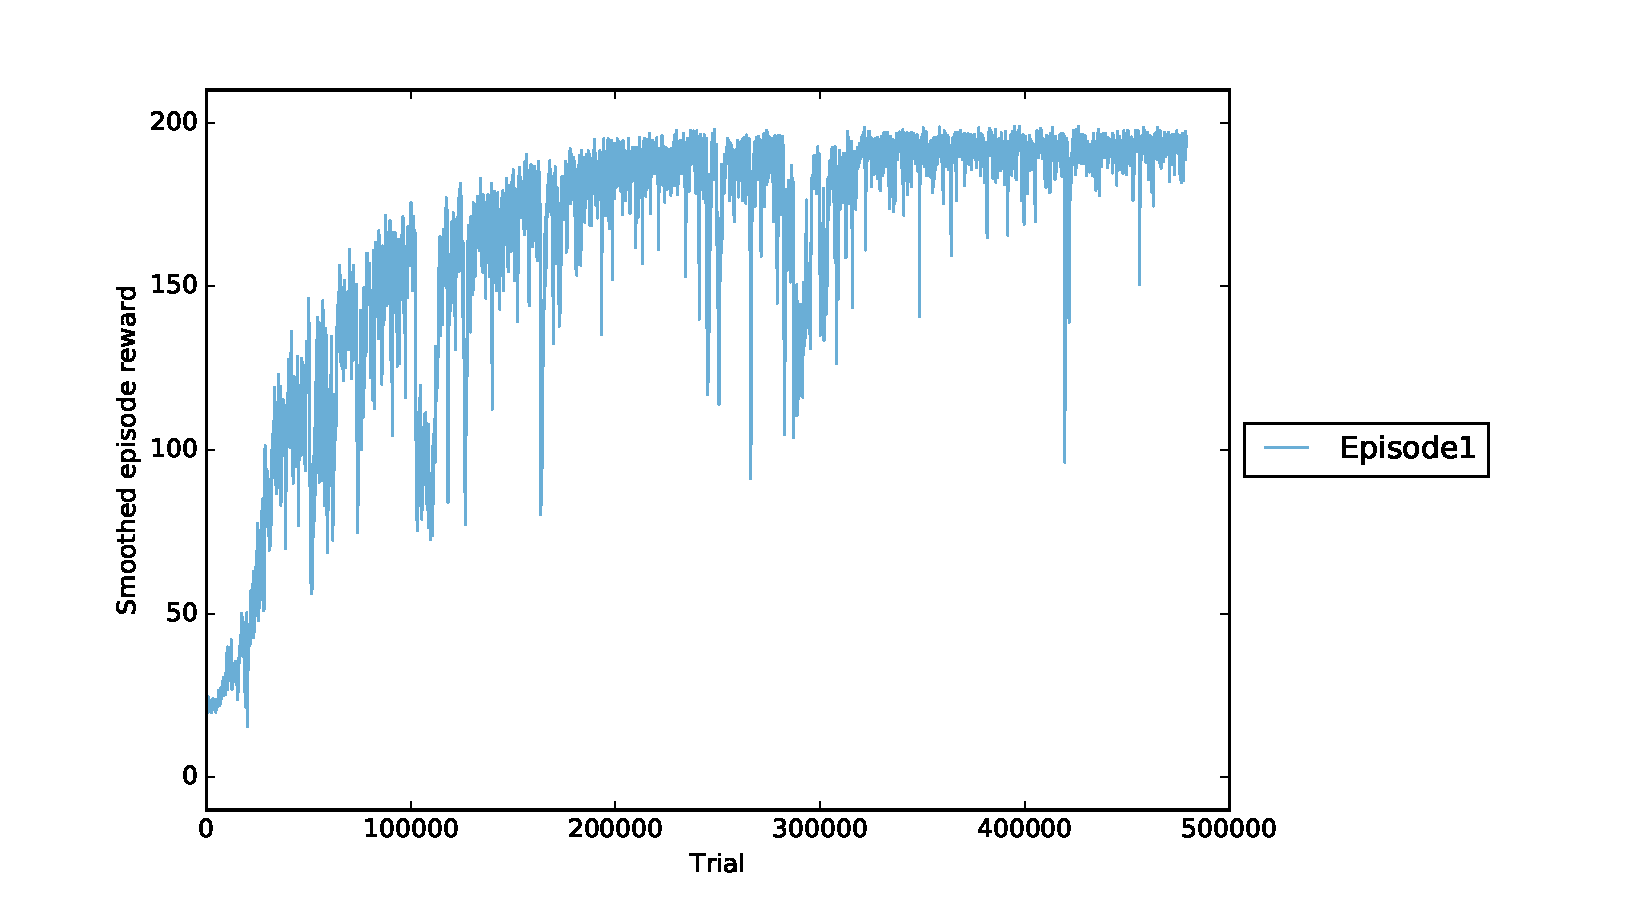
\includegraphics[width=0.49\linewidth]{fig/20permsLR1ep_training.pdf}}
	\subfloat[][Training over 2 episodes]{
		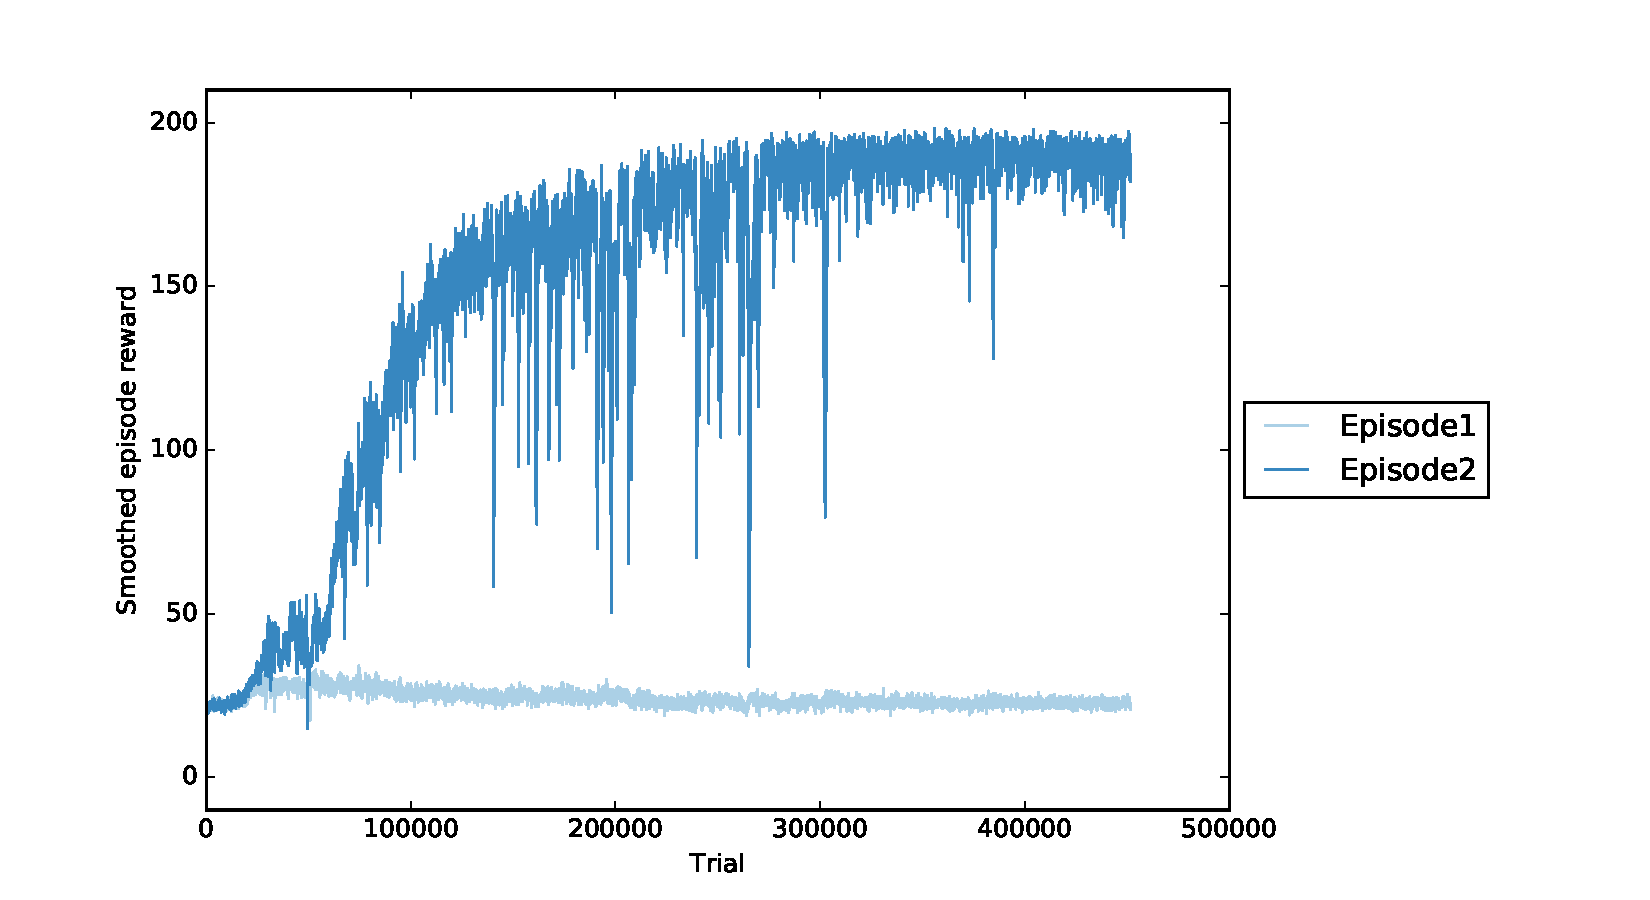
\includegraphics[width=0.49\linewidth]{fig/20permsLR2ep_training.pdf}}
	\\
	\subfloat[][Training over 3 episodes]{
		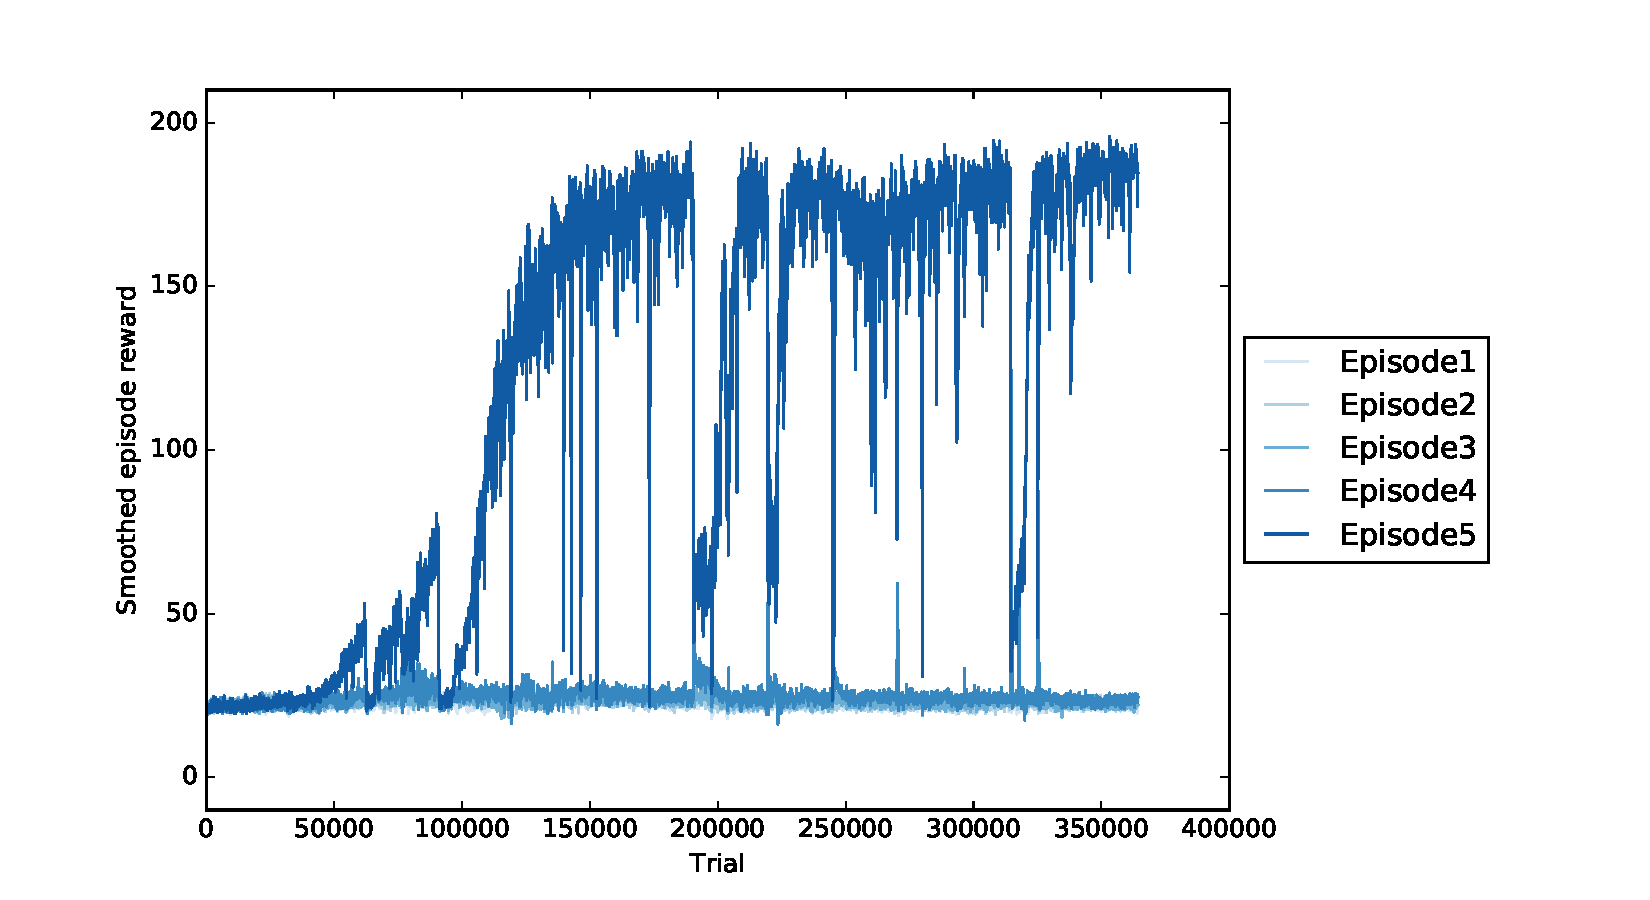
\includegraphics[width=0.9\linewidth]{fig/20permsLR5ep_training.pdf}}
	\caption{}
	\label{fig:20permsLR_training}
\end{figure}

\begin{figure}
	\centering
	\subfloat[][2 episodes]{
		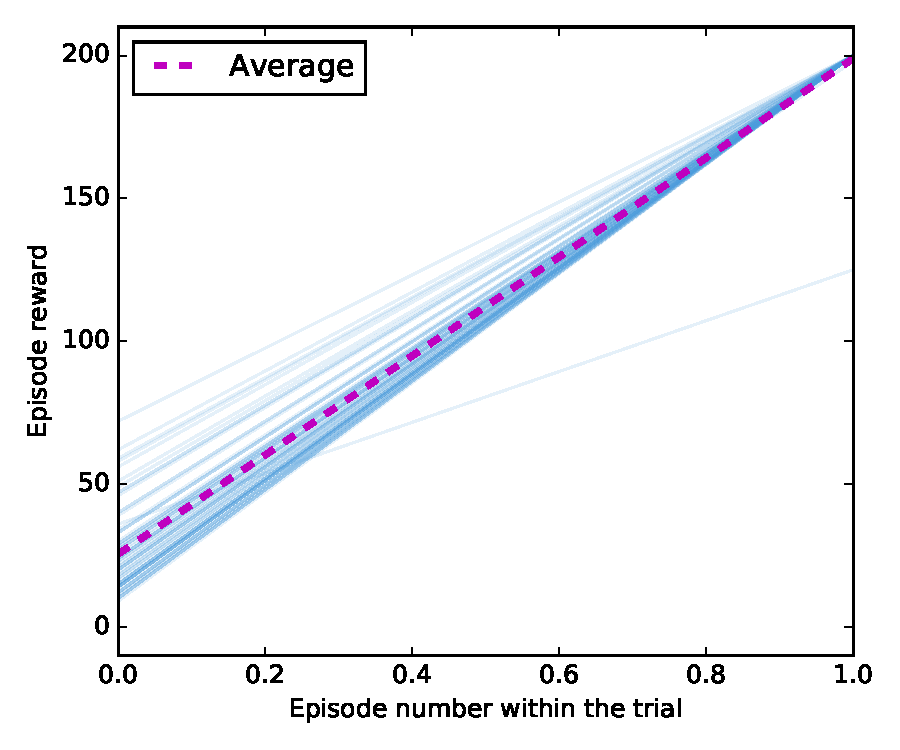
\includegraphics[width=0.33\linewidth]{fig/20permsLR2ep_rewards.pdf}}
	\subfloat[][5 episodes]{
		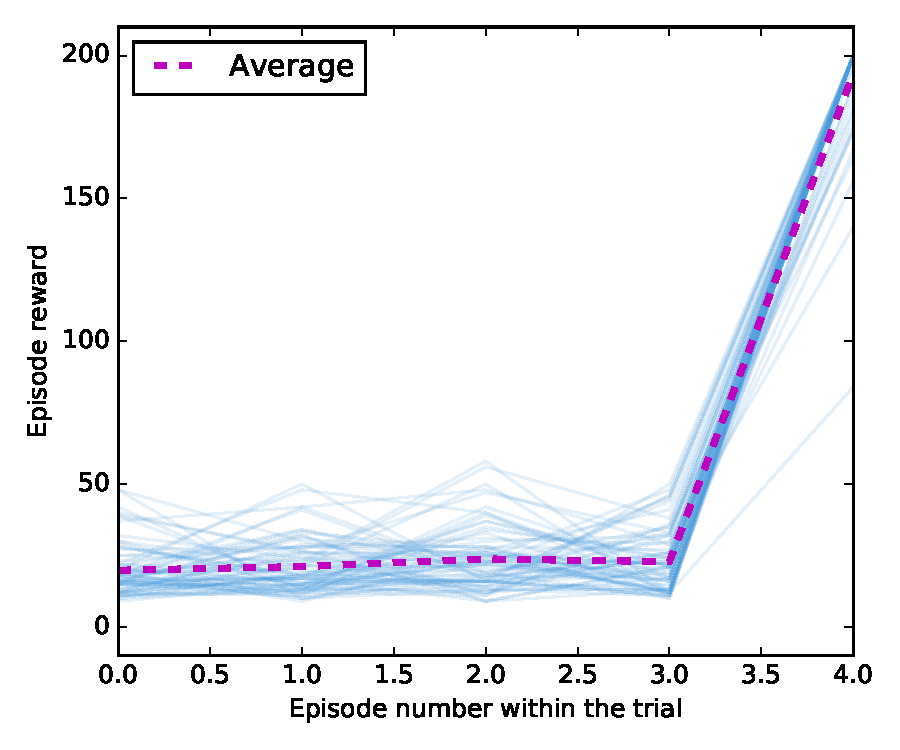
\includegraphics[width=0.33\linewidth]{fig/20permsLR5ep_rewards.pdf}}
	\subfloat[][10 episodes]{
		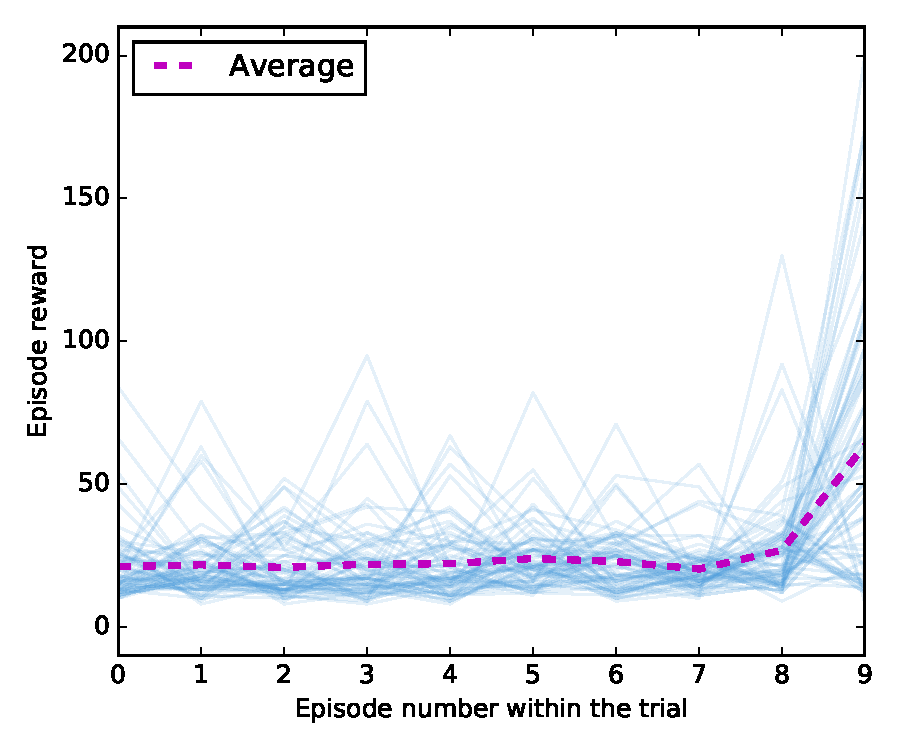
\includegraphics[width=0.33\linewidth]{fig/20permsLR10ep_rewards.pdf}}
	\caption{}
	\label{fig:20permsLR_rewards}
\end{figure}

\begin{figure}
	\centering
	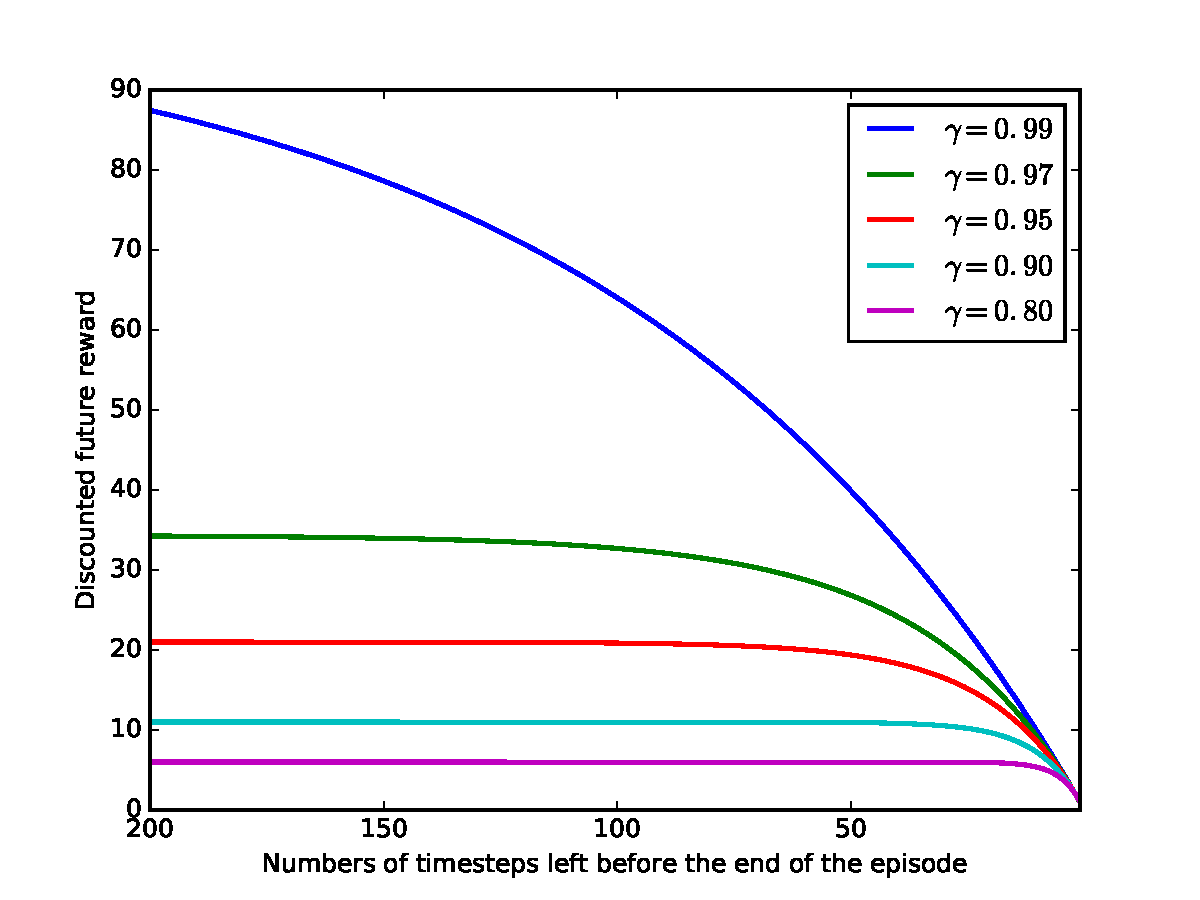
\includegraphics[width=0.8\linewidth]{fig/gamma_impact.pdf}
	\caption{}
	\label{fig:gamma_impact}
\end{figure}

\section{Problems with a 1-per-timestep reward}

\section{Tuning discount factor}
Show different gammas

\begin{figure}
	\centering
	\subfloat[][$\gamma=0.82$]{
		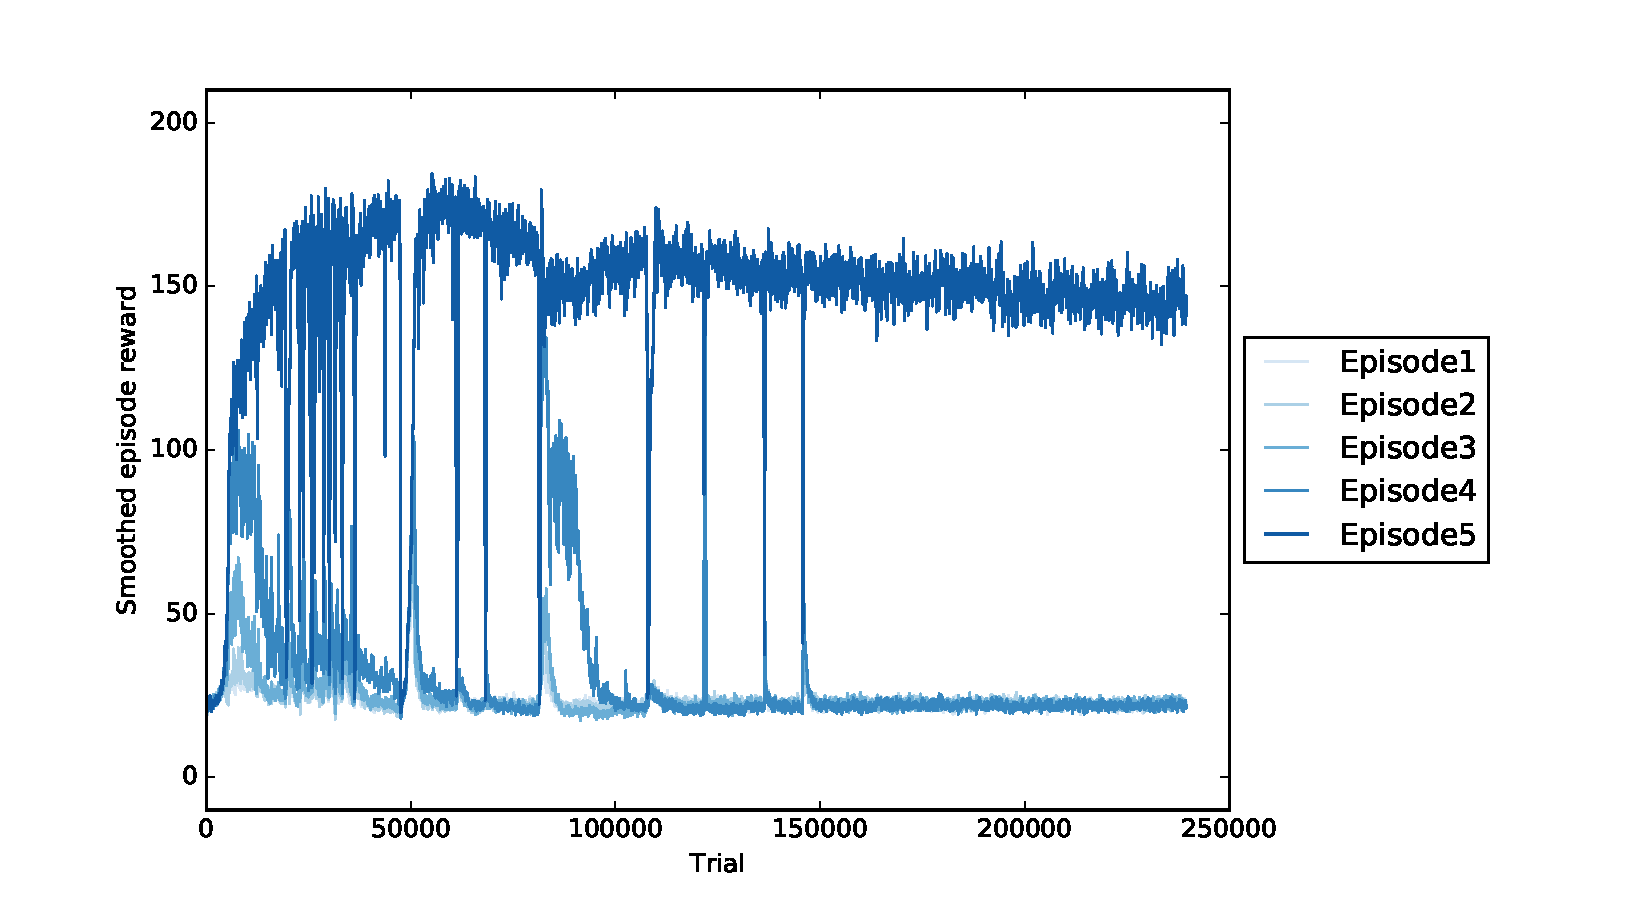
\includegraphics[width=0.49\linewidth]{fig/res_perms5ep_82.pdf}}
	\subfloat[][$\gamma=0.85$]{
		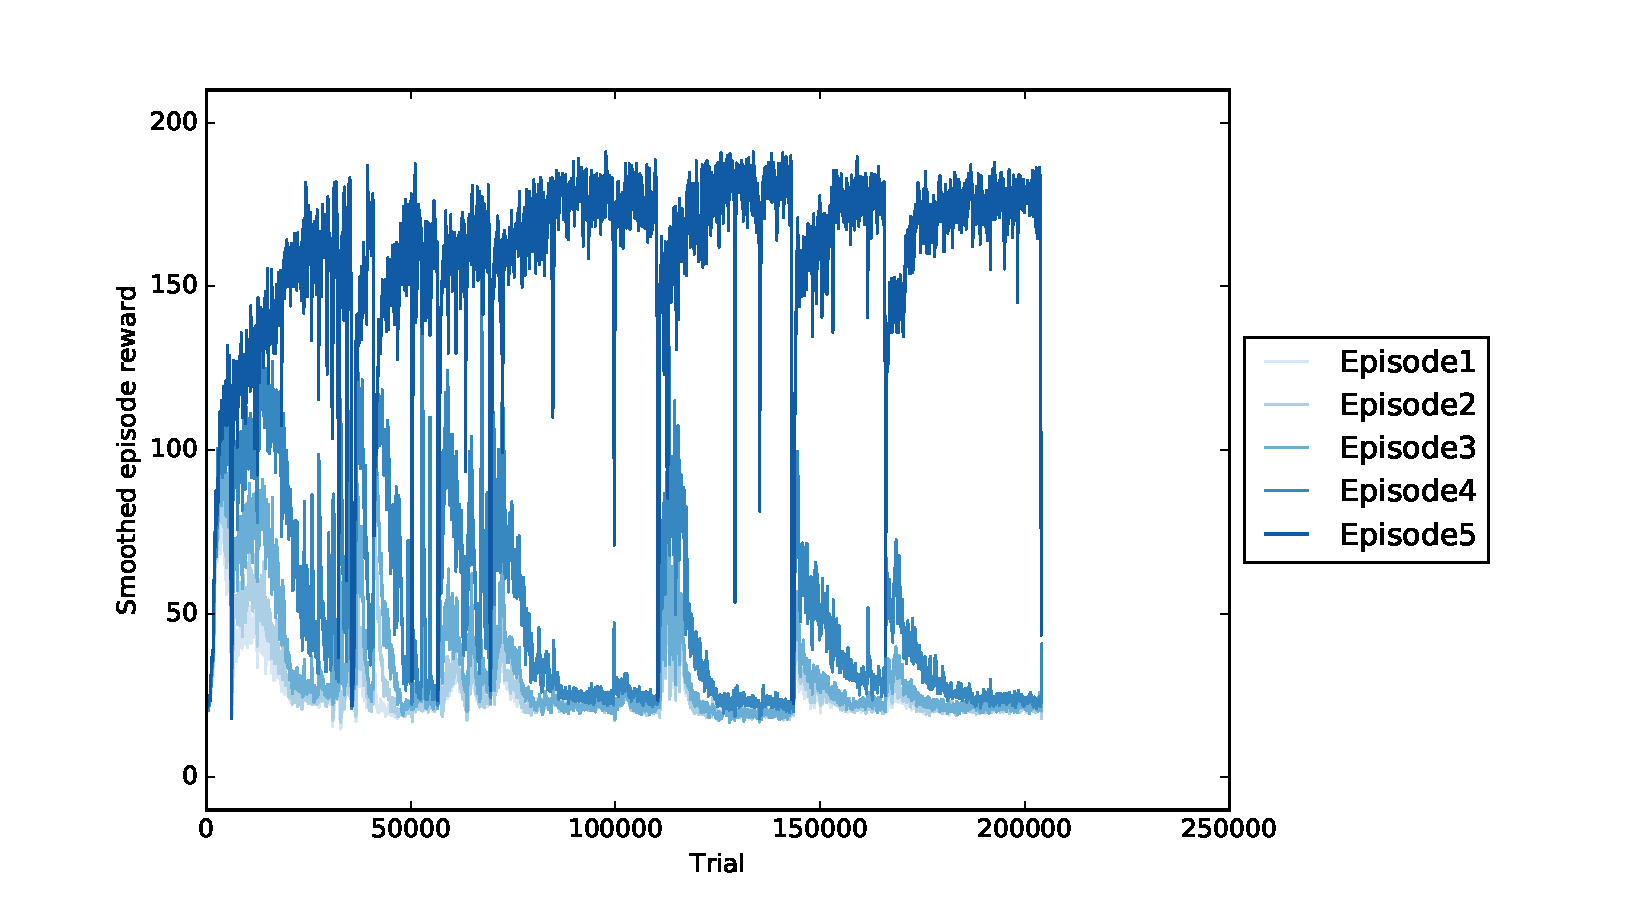
\includegraphics[width=0.49\linewidth]{fig/res_perms5ep_85.pdf}}
	\\
	\subfloat[][$\gamma=0.88$]{
		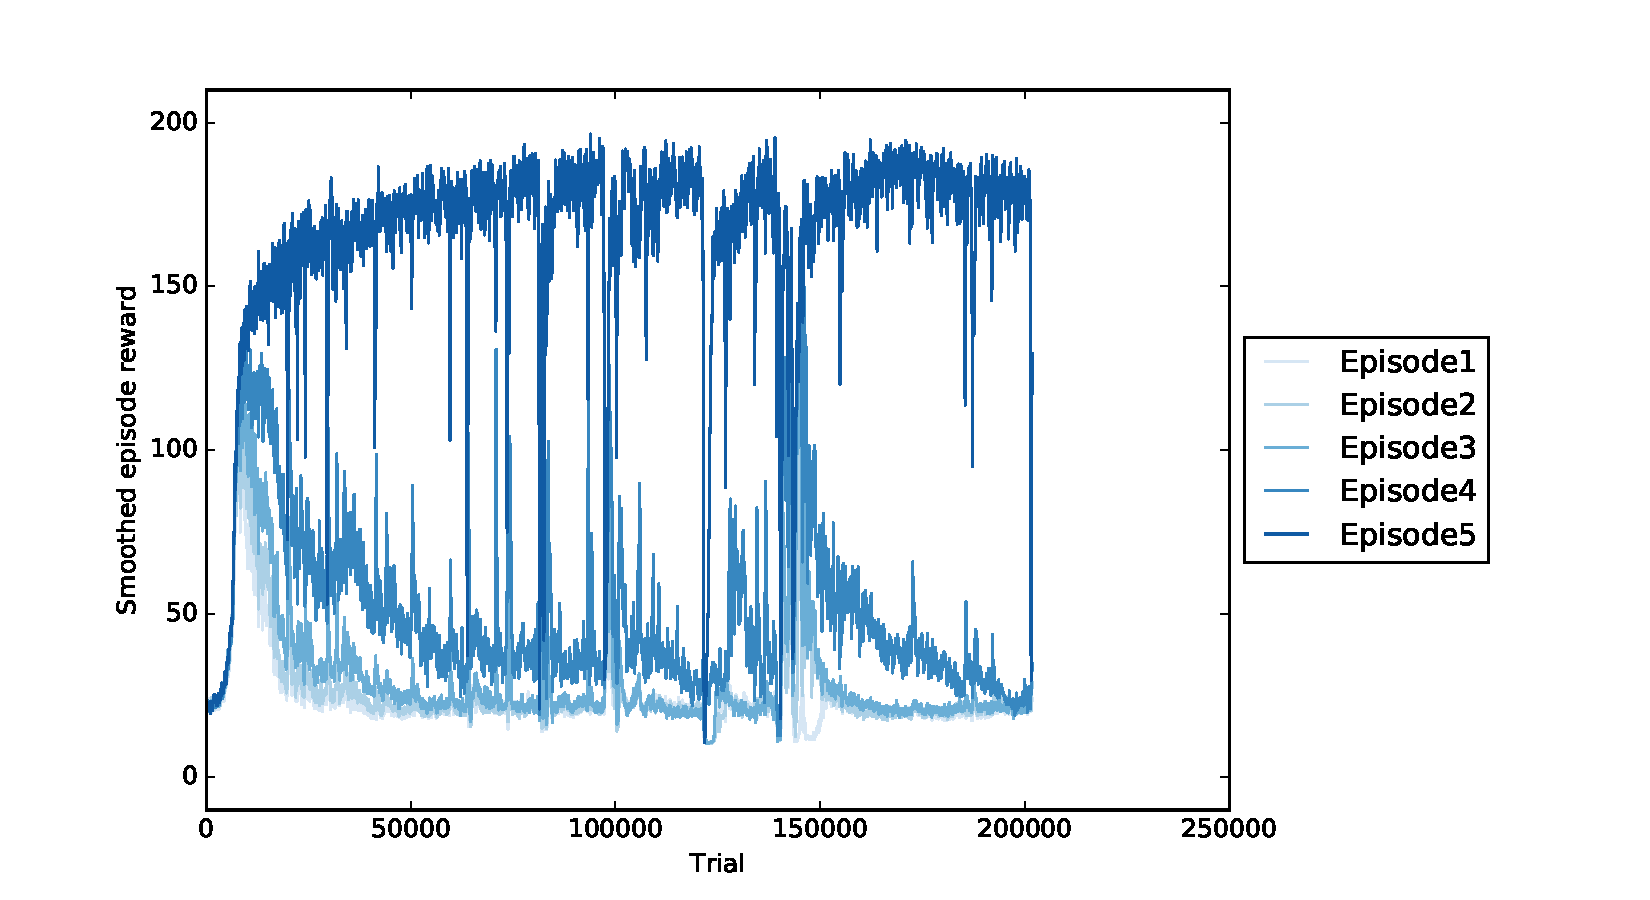
\includegraphics[width=0.49\linewidth]{fig/res_perms5ep_88.pdf}}
	\subfloat[][$\gamma=0.91$]{
		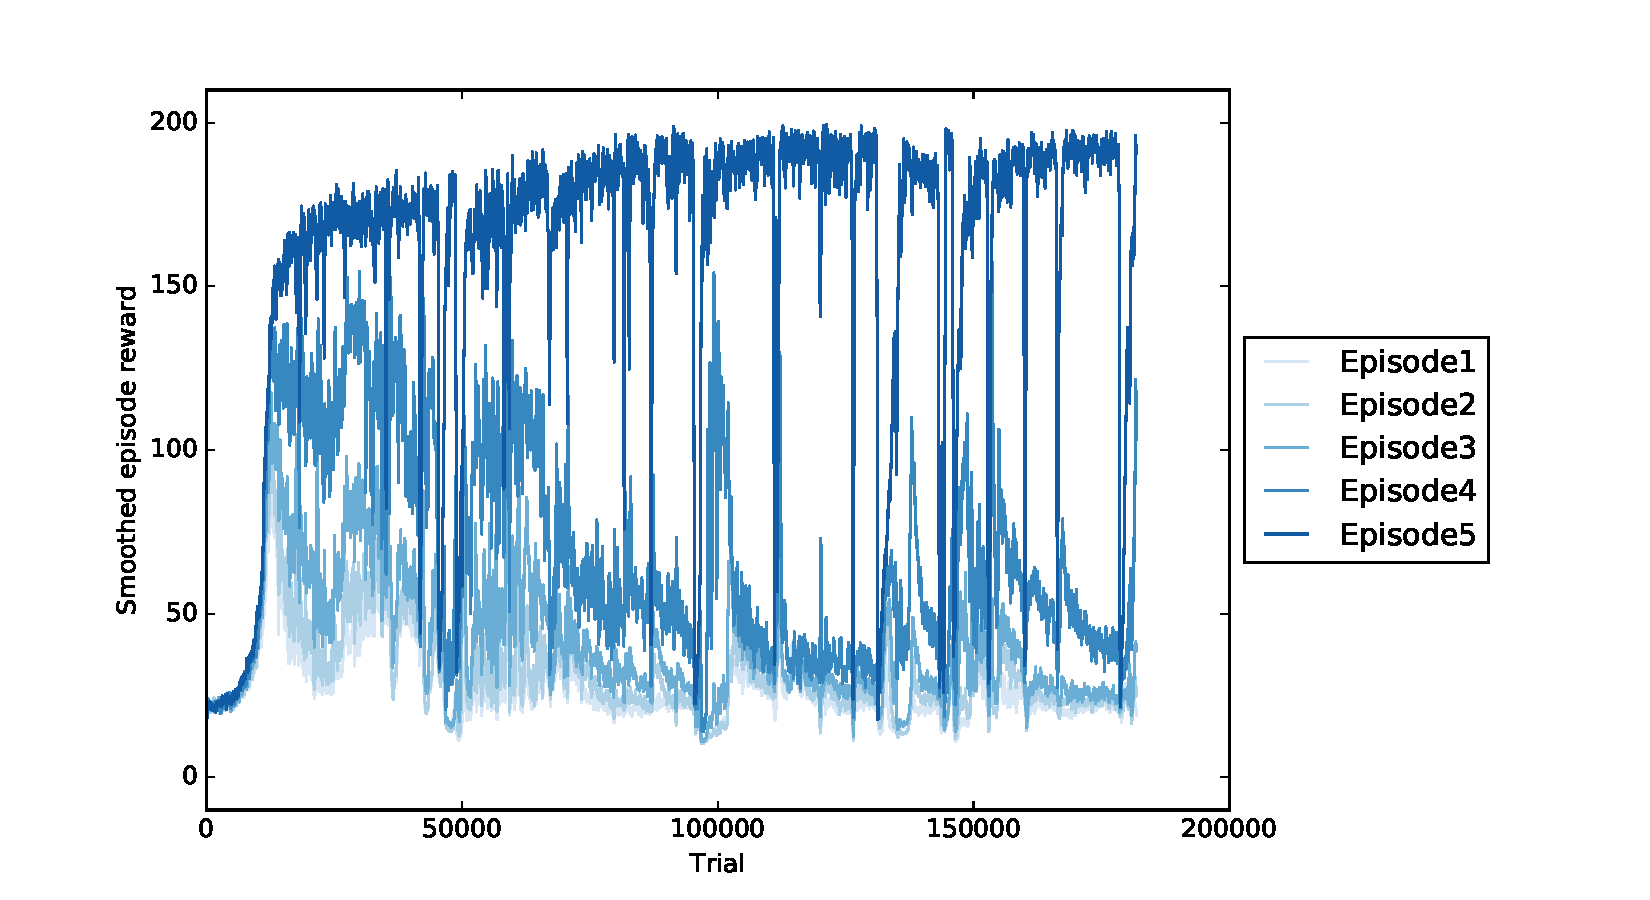
\includegraphics[width=0.49\linewidth]{fig/res_perms5ep_91.pdf}}
	\\
	\subfloat[][$\gamma=0.94$]{
		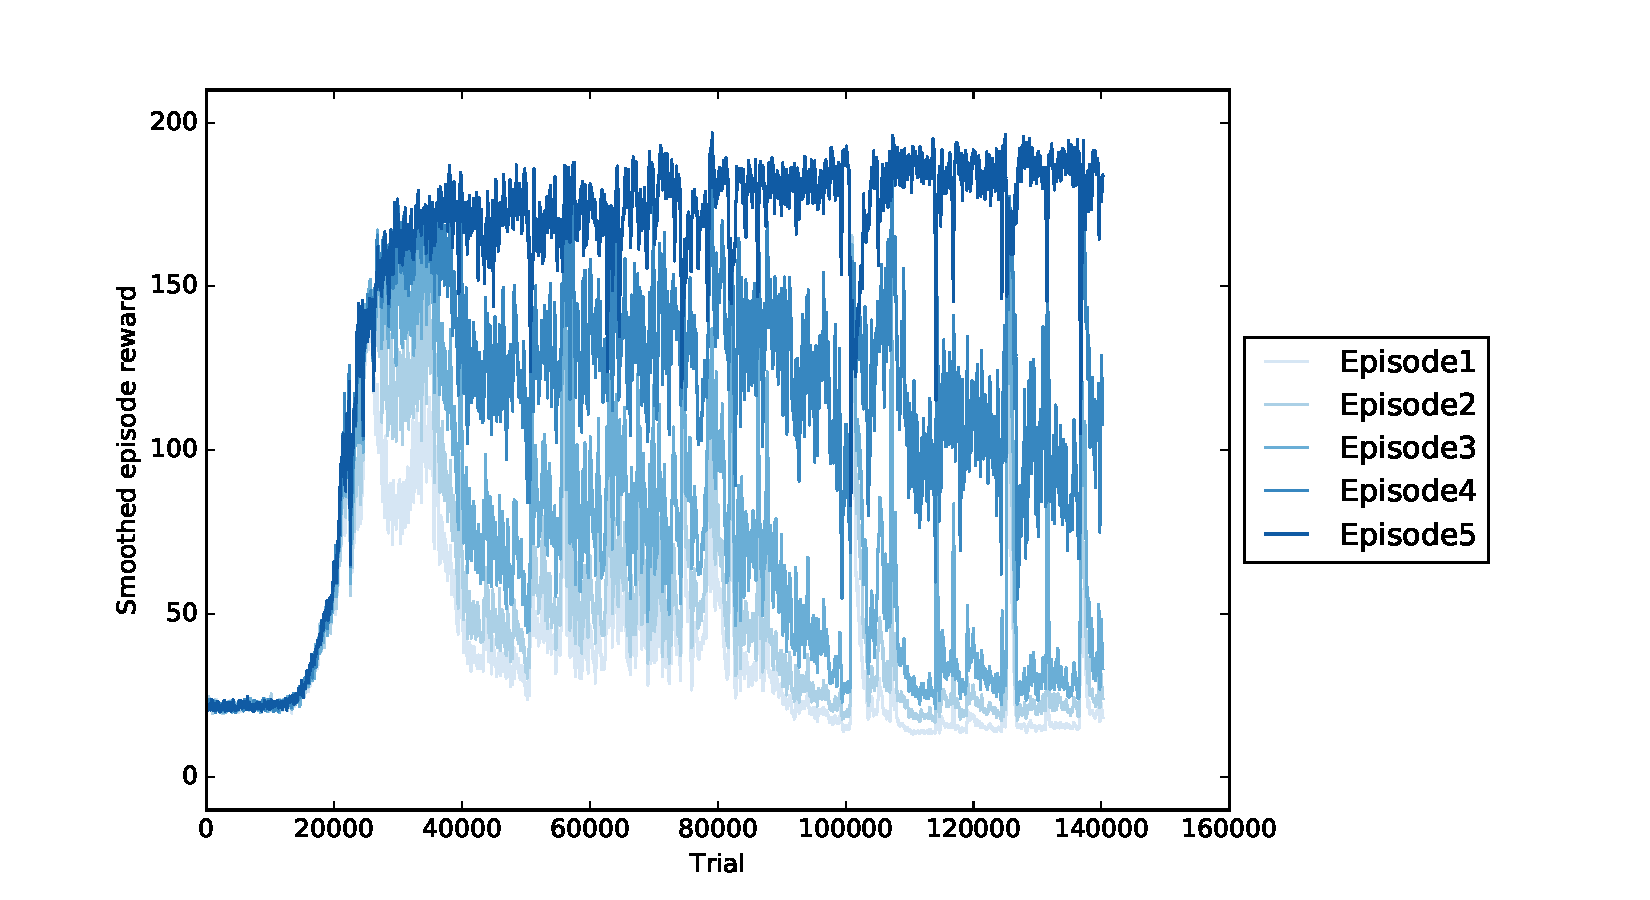
\includegraphics[width=0.49\linewidth]{fig/res_perms5ep_94.pdf}}
	\subfloat[][$\gamma=0.97$]{
		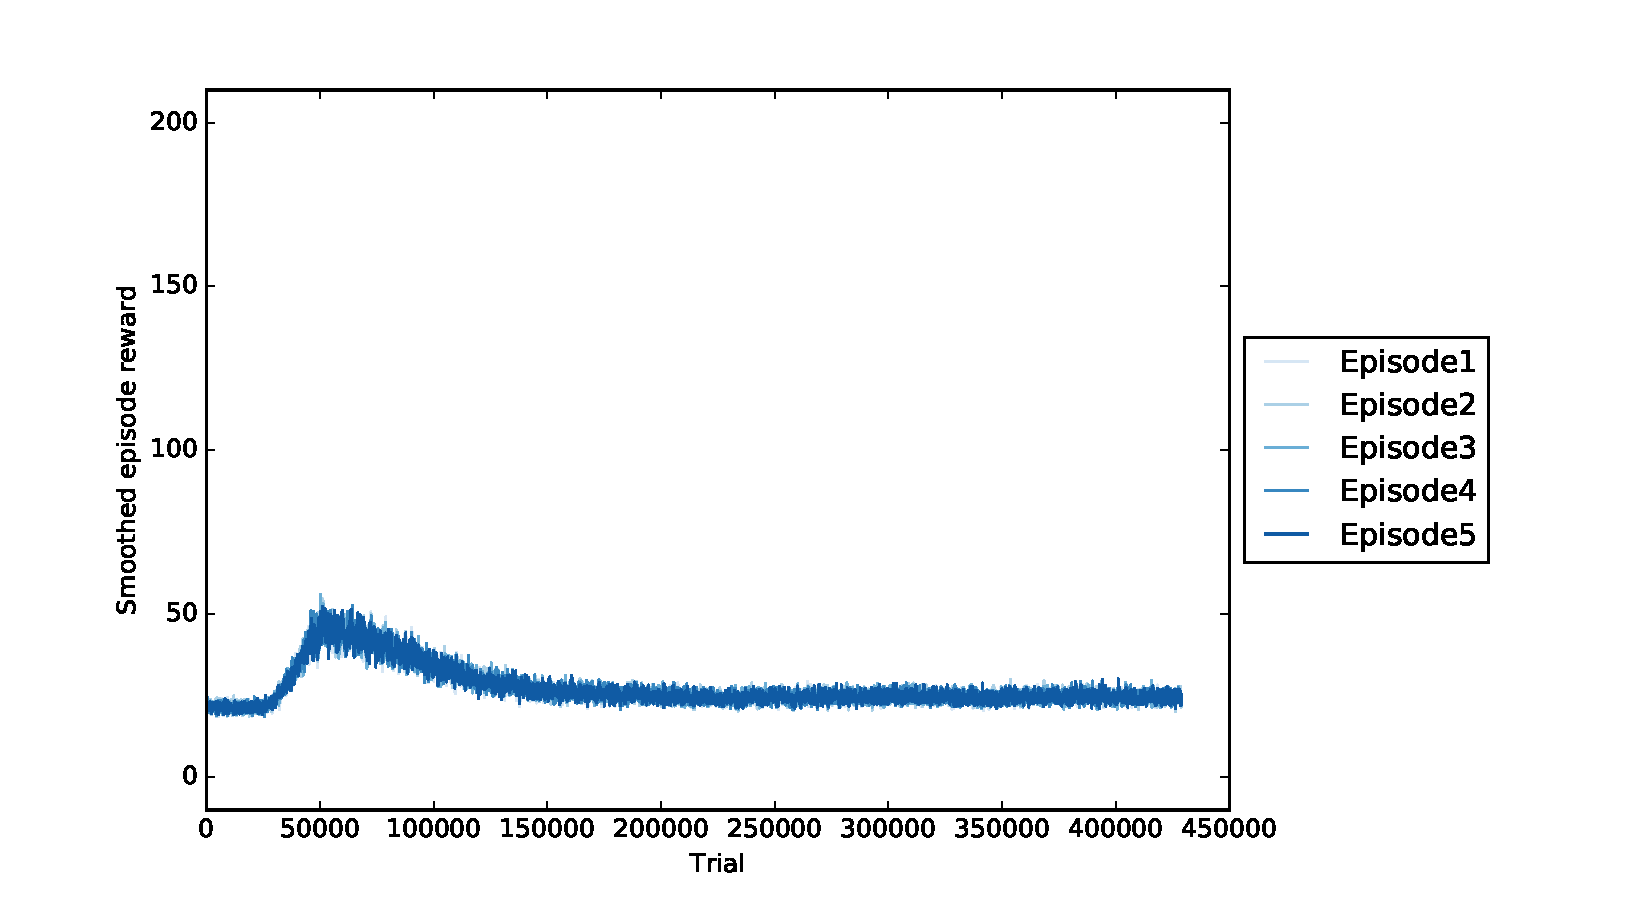
\includegraphics[width=0.49\linewidth]{fig/res_perms5ep_97.pdf}}
	\\
	\caption{}
	\label{fig:varied_gamma}
\end{figure}


